\documentclass[aps,prl,twocolumn,superscriptaddress,floatfix,nolongbibliography]{revtex4-2}
\usepackage{graphicx}
\graphicspath{{../figures/}}
\usepackage{amsmath,amssymb}
\usepackage{bm}
\usepackage[colorlinks=true,allcolors=blue]{hyperref}

\newcommand{\Fz}{F_0}
\newcommand{\PhiB}{\Phi_{\rm B}}
\newcommand{\Eg}{E_g}

\begin{document}

\title{Sub-cycle rectification at the metal contact in antenna-enhanced\\ high-harmonic generation from solids}

% TODO(authors): complete the author list and affiliations before submission.
\author{[Author list to be completed]}
\affiliation{[Affiliation to be completed]}

\date{\today}

\begin{abstract}
Metallic nanoantennas are used to enhance high-harmonic generation in solids and are modeled as
passive concentrators of the driving field. We show that this picture fails when the metal touches
the crystal. Real-space simulations of a metal--semiconductor junction in an antenna near field,
including the self-consistent space-charge field, show that electrons tunnel through the Schottky
barrier during one half-cycle only. The injected charge sheet, of order $10^{13}$~cm$^{-2}$,
screens up to half of the field in that half-cycle, enhances it in the other, and leaves a
quasistatic bias of up to 30\% of the driving amplitude. As a result even harmonics become as
strong as odd ones, harmonics below the band gap grow by up to two orders of magnitude, the
highest odd harmonics are suppressed, and the energy deposited per pulse rises by up to two orders
of magnitude.
An insulating spacer of half a nanometer removes all of these effects.
\end{abstract}

\maketitle

High-harmonic generation (HHG) in crystals~\cite{ghimire2011,ghimire2019,vampa2014} requires
fields of order 1~V/nm, close to the damage threshold of most materials. Plasmonic nanoantennas
reach such fields in nanoscale hot spots at incident intensities one to two orders of magnitude
lower, an idea first pursued in gases~\cite{kim2008,sivis2013} and now established for
solids: gold antennas on silicon~\cite{vampa2017,jalil2023} and
ZnO~\cite{imasaka2018}, metal-coated sapphire cones~\cite{han2016}, and dielectric
counterparts~\cite{sivis2017,liu2018,tonkaev2026}. In every theoretical
description so far the metal enters only through the field it produces: an enhanced, spatially
inhomogeneous but otherwise prescribed driving field acting on the bulk
response of the crystal~\cite{ciappina2012,husakou2011,rudenko2022}.

This description overlooks where the hot spot sits. Field enhancement is largest at the edges of
the antenna, that is, at a metal--semiconductor contact. There the metal Fermi level lies inside
the gap, and an electron needs to cross only the Schottky barrier $\PhiB$, typically below
1~eV~\cite{tersoff1984}, rather than the gap $\Eg$. Tunneling rates depend exponentially
on the barrier height to the power $3/2$~\cite{fowler1928,keldysh1965}, so a contact
should emit carriers at fields far below the onset of interband
tunneling. Optical-field-driven tunneling from metal nanostructures into vacuum or across
nanogaps is well documented~\cite{kruger2011,rybka2016,putnam2017}, and
charge transfer across metal--semiconductor interfaces occurs within hundreds of
attoseconds~\cite{heide2020}. Recently, field-driven tunneling currents from gold nanoantennas
into silicon were measured under mid-infrared excitation~\cite{li2023}. In the HHG context,
Imasaka \textit{et al.} observed band-gap fluorescence with an anomalously weak intensity
dependence from ZnO under gold antennas and conjectured carrier transfer from the
metal~\cite{imasaka2018}. Whether, and how, such injection alters harmonic generation has
not been examined.

\begin{figure*}
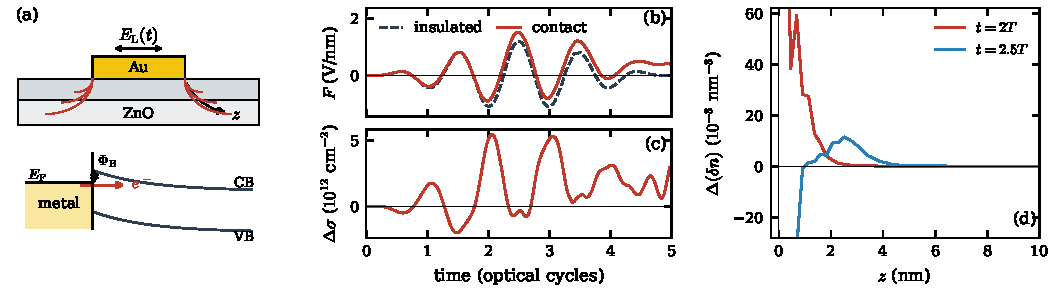
\includegraphics[width=\textwidth]{fig1.pdf}
\caption{(a) Geometry and band alignment: the hot spot of an antenna sits at a metal--semiconductor
contact, where electrons need to tunnel only through the Schottky barrier $\PhiB$. (b) Field
inside the crystal for the contacted (solid) and insulated (dashed) junction at
$\Fz=1.0$~V/nm. (c) Induced electron charge in the crystal beyond the first two unit cells
in excess of the insulated case; it is screened and thus smaller than the free charge of
Eq.~\eqref{eq:gauss} by about the factor $\varepsilon$. (d) Cell-averaged induced electron
density in excess of the insulated case at a forward ($t=2T$) and the following reverse
($t=2.5T$) field extremum; the feature at $z\approx0$ (off scale) is the screening charge of
the metal.}
\label{fig1}
\end{figure*}

In this Letter we show that it does so profoundly. The contact behaves as a tunnel diode loaded
by the capacitance of the crystal: charge injected during one half-cycle generates a space-charge
field that clips that half-cycle and biases the next. The near field inside the crystal thereby
loses its half-wave symmetry, with direct consequences for the harmonic spectrum, for the
energy deposited in the hot spot, and for the interpretation of existing experiments.

\textit{Model.}---We consider the dynamics along the field line that leaves the edge of the
contact [Fig.~\ref{fig1}(a)], with coordinate $z$ pointing from the metal ($z<0$) into the crystal.
Electrons obey (atomic units)
\begin{equation}
i\partial_t\psi_j=\Big[-\tfrac12\partial_z^2+V(z)+D(t)\,g(z)+U_{\rm H}(z,t)\Big]\psi_j .
\label{eq:tdse}
\end{equation}
The static potential $V$ consists of a jellium metal with Fermi energy 5.5~eV, a crystal
described by the Mathieu potential $-V_0[1+\cos(2\pi z/a)]$~\cite{wu2015} with $a=0.42$~nm and
$V_0$ chosen to give a gap $\Eg=3.34$~eV between the second and third bands, and vacuum beyond
(electron affinity 4~eV). All eigenstates below the Fermi level $E_{\rm F}=E_c-\PhiB$ are occupied,
with $\PhiB=0.7$~eV unless stated otherwise; this includes the metal-induced gap states that
form at the interface~\cite{tersoff1984}. The antenna's oscillating surface charge is
represented by an external sheet at the metal surface whose field decays into the crystal over
the near-field length $\ell=8$~nm: $g(z)=\ell(1-e^{-z/\ell})$ for $z>0$ and $g=0$ in the metal.
The driver, $D(t)=D_0\sin^2(\pi t/\tau)\cos\omega t$, has wavelength $2.1~\mu$m
($\hbar\omega=0.59$~eV, $\Eg=5.7\hbar\omega$) and total duration $\tau$ of five cycles.

The term $U_{\rm H}$ is essential. It is the Hartree potential of the induced density
$\delta n$ in planar geometry, $\partial_z^2U_{\rm H}=-4\pi\,\delta n$, with two electrons per
orbital and one chain per area $a^2$. It accounts for the dielectric response of the valence
electrons, the screening by the metal, and the field of any injected charge. Because the valence
electrons screen $D$, we characterize the excitation by the field inside the crystal, $F(t)$,
defined as the gradient of $Dg+U_{\rm H}$ averaged over the first four unit cells
beyond the interface layer (0.4 to 2.1~nm). As reference we use the same system with a
1.5-nm insulating spacer (barrier 3.1~eV above $E_c$, permittivity 3.9, as for
SiO$_2$) between metal and crystal, which suppresses tunneling but leaves the field unchanged.
The peak of $F$ in this ``insulated'' configuration defines $\Fz$; it corresponds to an
effective permittivity $D_0/\Fz\simeq5.6$. Equation~\eqref{eq:tdse} is propagated for all
occupied orbitals with a split-operator scheme~\cite{SM}. Emission is obtained from the total
current, $S(\Omega)\propto|\int\!dt\,w(t)\,\dot J(t)e^{i\Omega t}|^2$ with a Hann window $w$.
Related models describe bulk and impurity-assisted HHG~\cite{wu2015,yu2019}; new here are
the metal reservoir and the self-consistent field.

\begin{figure}
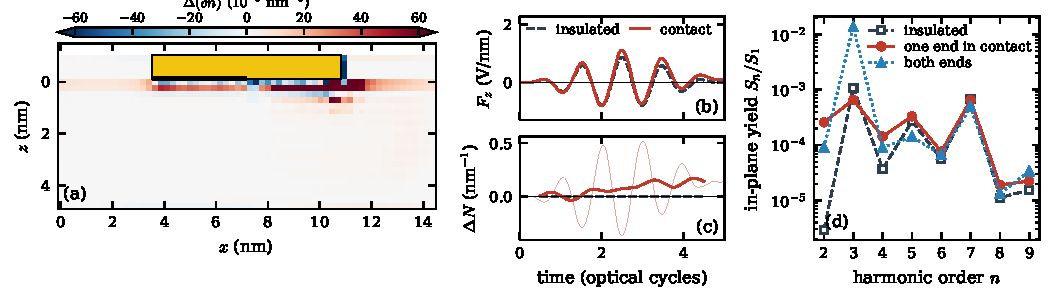
\includegraphics[width=\columnwidth]{fig2.pdf}
\caption{Harmonic yields of the contacted (circles) and insulated (squares) junction for
(a) $\Fz=1.0$~V/nm and (b) $\Fz=1.4$~V/nm, normalized to the fundamental of the insulated
case. The shaded region marks photon energies above the band gap.}
\label{fig2}
\end{figure}

\textit{Rectification of the near field.}---Figure~\ref{fig1}(b) compares $F(t)$ for the
contacted and the insulated junction at $\Fz=1.0$~V/nm. Without tunneling the field is
symmetric. With the contact, the half-cycles in which the force on the electrons points into
the crystal (forward) are clipped to $F_-=0.52$~V/nm, the reverse half-cycles are enhanced to
$F_+=1.28$~V/nm, and a field of 0.2 to 0.5~V/nm persists at the zero crossings of the
driver and after the pulse. The origin is seen in Figs.~\ref{fig1}(c) and \ref{fig1}(d). During each
forward half-cycle electrons tunnel from the metal into the conduction band and form a sheet
that extends a few nanometers into the crystal; its field opposes the driver, which
self-limits the injection. When the driver reverses, conduction electrons can return to the
metal without a barrier, but valence electrons face the much larger barrier $\Eg-\PhiB$, so no
compensating hole sheet forms. Part of the injected charge moves deeper into the crystal instead
of returning [Fig.~\ref{fig1}(d)], and its field adds to the driver in the reverse half-cycle.
The crystal therefore carries a net negative charge throughout the pulse
[Fig.~\ref{fig1}(c)]. The sheet density of free charge follows from Gauss's law,
\begin{equation}
\sigma\simeq\varepsilon\varepsilon_0\,\Delta F/e ,
\label{eq:gauss}
\end{equation}
which gives $\sigma\approx1.5\times10^{13}$~cm$^{-2}$ for the clipped amplitude
$\Delta F=\Fz-F_-$ and $0.9\times10^{13}$~cm$^{-2}$ for the quasistatic component
$F_{\rm dc}=0.29$~V/nm, defined as the average of $F$ over the two central cycles. This is a
third to a half of the surface charge density $\varepsilon_0D_0/e$ of the antenna itself.
Equation~\eqref{eq:gauss} also states the limit of the effect: the injected charge can at most
cancel the forward field, in which case the waveform would oscillate between 0 and $2\Fz$, as
in an electronic clamping circuit.

\begin{figure*}
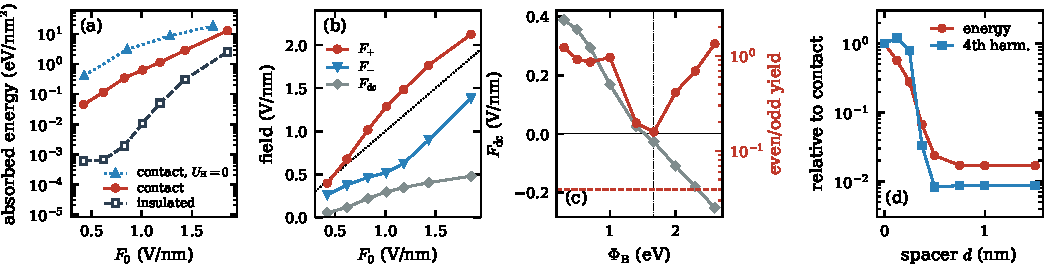
\includegraphics[width=\textwidth]{fig3.pdf}
\caption{(a) Energy absorbed per unit contact area versus driving field for the contacted
and insulated junction, and for the contacted junction without the space-charge field.
(b) Peak field in the reverse ($F_+$) and forward ($F_-$) half-cycles and
quasistatic component $F_{\rm dc}$; the dotted line is the insulated case. (c) Quasistatic
field (diamonds, left axis) and even-to-odd yield ratio (circles, right axis) versus Schottky
barrier at $\Fz=1.0$~V/nm; the vertical line marks midgap and the dashed line the even-to-odd
ratio of the insulated junction. (d) Absorbed energy and fourth-harmonic yield versus the
thickness $d$ of an insulating spacer, relative to the contacted junction.}
\label{fig3}
\end{figure*}

The dependence on the driving amplitude is shown in Fig.~\ref{fig3}(b). Between
$\Fz=0.4$ and 1.85~V/nm the forward half-cycle is reduced to 51\%--75\% of $\Fz$, the reverse
one is enhanced by up to 27\%, and $F_{\rm dc}$ amounts to 12\%--29\% of $\Fz$.

\textit{Harmonic spectrum.}---A waveform without half-wave symmetry drives even harmonics
in a centrosymmetric medium, and a quasistatic field does so already through the bulk
response~\cite{vampa2018}. Figure~\ref{fig2} shows the harmonic yields. In the insulated
junction the even orders lie one to two orders of magnitude below the odd ones; the remainder
stems from the surface of the crystal and from the field gradient~\cite{ciappina2012,vampa2017}.
With the contact, even and odd harmonics have comparable strength. At $\Fz=1.0$~V/nm the
fourth and sixth harmonics grow by factors of 120 and 68, and the ratio of even (fourth plus
sixth) to odd (third plus fifth) yield rises from 0.04 to 0.9; it stays between 0.9 and 1.5 for
all $\Fz\ge0.8$~V/nm. The contact also redistributes the odd orders. Harmonics below the gap
are enhanced, the fifth by a factor of 35, because the rectified injection current is itself a
source of low-order radiation, in the manner of Brunel and injection-current
harmonics~\cite{brunel1990,jurgens2020,babushkin2025}. The highest odd harmonics, in contrast, are reduced, the ninth by a factor of 37 at this
field. We attribute the reduction to the quasistatic bias,
which makes successive half-cycles inequivalent for the interband polarization, and to the loss of
recolliding carriers into the metal~\cite{husakou2011}. At $\Fz=1.4$~V/nm, where interband
excitation is strong, the yields of the two junctions approach each other above the gap while
the enhancement below it persists [Fig.~\ref{fig2}(b)].

\textit{Energy deposition and space charge.}---Figure~\ref{fig3}(a) shows the energy absorbed
per unit contact area. In the insulated junction absorption is governed by interband
excitation and rises steeply with field. The contact opens a channel with a much weaker field
dependence: the absorbed energy is larger by a factor of 60 at $\Fz=1.0$~V/nm and by up to
180 at lower fields, and the two curves approach each other only near 2~V/nm. The enhanced
reverse half-cycle also promotes interband excitation: the
density of valence-band holes left after the pulse, a prerequisite for band-gap
fluorescence, is 14 times larger than in the insulated junction at $\Fz=1.0$~V/nm. Space
charge is decisive for all of these numbers. If $U_{\rm H}$ is switched off, the absorbed energy
is larger by another order of magnitude [triangles in Fig.~\ref{fig3}(a)] and the field is, by
construction, not rectified. Independent-electron descriptions therefore overestimate the
injection and miss its main consequence.

\textit{Control parameters.}---Two parameters identify the mechanism. The first is the
barrier height [Fig.~\ref{fig3}(c)]. As the Fermi level is moved from the conduction-band
side toward midgap, the quasistatic field decreases and vanishes at
$\PhiB\simeq\Eg/2$, where electron and hole injection balance; beyond midgap it changes
sign because holes are now injected preferentially. The even-to-odd ratio follows, with a
minimum at midgap. The second parameter is the separation $d$ between metal and
crystal [Fig.~\ref{fig3}(d)]. An insulating layer of 0.25~nm reduces the absorbed energy by
a factor of 3.6; at 0.5~nm rectification and even harmonics are gone, and from 0.75~nm on
the response is indistinguishable from that of the crystal without any metal. The
near-field enhancement, in contrast, varies on the scale of the antenna's radius of
curvature and is unaffected by such a layer.

\textit{Implications for experiments.}---In antennas lying on a substrate the contact edge
coincides with the hot spot, and the field lines leaving it have components both normal
and parallel to the surface. The parallel component of the injection current radiates into
the surface normal, where harmonics are usually collected. For an antenna with mirror
symmetry the two ends are driven half a cycle apart with opposite outward normals, so
their contributions to the $n$th harmonic carry the relative sign $(-1)^{n+1}$~\cite{SM}: odd
orders add, whereas even orders cancel on axis and appear only off axis or for asymmetric
antennas. This is the same far-field rule as for the field-gradient
mechanism~\cite{vampa2017}. It is consistent with the absence of structure-induced even
harmonics for rod antennas~\cite{vampa2017,imasaka2018} and with their observation for
triangular ones~\cite{jalil2023}, which was attributed to the gradient. Our results show
that a contact generates even harmonics far more efficiently than surface and gradient
together, and they provide a test: a sub-nanometer oxide, or a metal whose Fermi level is
pinned near midgap, suppresses the contact contribution but not the gradient one. The same
test tells whether a given sample is in the contact regime at all, since native oxides and
adhesion layers decide whether the contact is intimate. Rectification also offers an
explanation for the band-gap fluorescence with a low-order intensity dependence seen only
under antennas on ZnO~\cite{imasaka2018}, and it implies a static field at
metal--semiconductor nanostructures that builds up within an optical cycle, in addition to the
slowly accumulating one inferred from second-harmonic generation~\cite{sun2023}. For odd
harmonics, part of the observed enhancement below the gap may be injection current, while
the highest harmonics can be weaker than a passive field-enhancement estimate predicts.
Finally, since the contact multiplies the deposited energy, a spacer should raise the damage
threshold of plasmonic HHG sources~\cite{sivis2013,vampa2017}.

Our model is deliberately minimal. It is one-dimensional, treats the electron--electron
interaction at the mean-field level, and contains no scattering, so that it applies to
few-cycle pulses; for longer pulses the quasistatic field grows from cycle to
cycle~\cite{SM} until back-flow and relaxation balance the injection. Adhesion layers,
interface states, and band bending are subsumed in $\PhiB$. The planar treatment of the
space charge requires the injected sheet to lie closer to the metal than the lateral size
of the hot spot, which holds here. The results are converged to within 15\%, and
rectification depends only weakly on the near-field decay length and the wavelength~\cite{SM}. None of these restrictions affects the
mechanism, which rests on the asymmetry between the barriers for electrons and holes and on
Gauss's law.

In summary, a metal antenna in contact with a semiconductor is not a passive field
concentrator. It injects a space-charge-limited sheet of carriers in every cycle, and the
field of that sheet rectifies the near field that drives the crystal. A spacer of half a
nanometer switches the effect off, which gives experiments a simple control and antenna
design a new degree of freedom: the contact can be removed where clean spectra and high
damage thresholds are wanted, or engineered through the barrier height where a built-in
sub-cycle bias is useful, for instance for even-harmonic generation in centrosymmetric
crystals or for lightwave-driven currents~\cite{schiffrin2013}.

% TODO(authors): add funding acknowledgments and the statement on the use of AI tools required by APS.
\begin{acknowledgments}
[Acknowledgments to be completed.]
\end{acknowledgments}

\textit{Data availability.}---The simulation code and the data are openly
available~\cite{repo}.

\bibliography{refs}

\end{document}
